%%%%%%%%%%%%%%%%%%%%%%%%%%%%%%%%%%%%%%%%%%%%%%%%%%%%%%%%%%%%%%%%%%%%%%%%
% Escuela Politécnica Superior de la Universidad de Alicante
% Realizado por: Jose Manuel Requena Plens
% Contacto: info@jmrplens.com / Telegram:@jmrplens
%%%%%%%%%%%%%%%%%%%%%%%%%%%%%%%%%%%%%%%%%%%%%%%%%%%%%%%%%%%%%%%%%%%%%%%%

\definecolor{mycolor1}{rgb}{1.00000,0.00000,1.00000}%
%
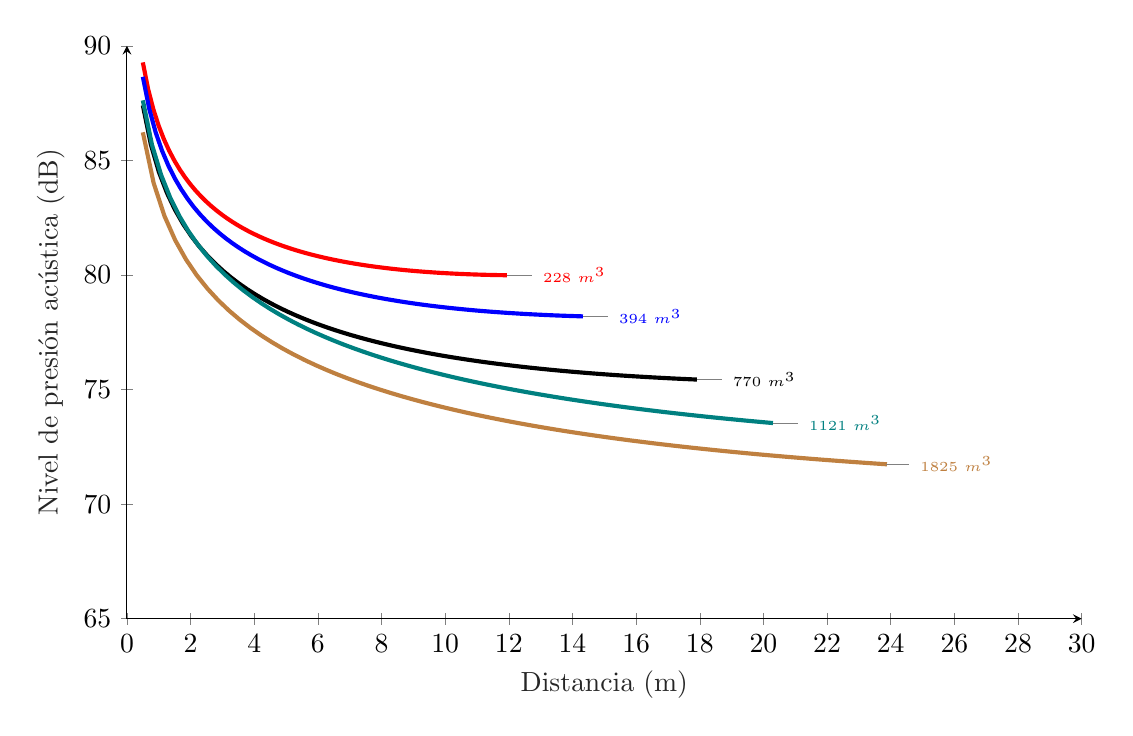
\begin{tikzpicture}

\begin{axis}[%
width=\textwidth,
height=0.6\textwidth,
at={(0\textwidth,0\textwidth)},
scale only axis,
xmin=0,
xmax=30,
xlabel style={font=\color{white!15!black}},
xlabel={Distancia (m)},
ymin=65,
ymax=90,
axis y line=left,
axis x line=bottom,
cycle list name=color list,
ylabel style={font=\color{white!15!black}},
ylabel={Nivel de presión acústica (dB)},
axis background/.style={fill=white},
legend style={legend cell align=left, align=left, draw=white!15!black}
]

% Capos utiles

% 1
\addplot+[ line width=1.5,domain=0.5:11.94, samples=70,every node/.style={xshift=-4pt}]
{10*log10(1.0337e+12 * ( ( 4*0.0026389378 / (272*(-ln(1-0.109))*x) * ( e^(-(13.82*(x/343)*(-2.209) / 1.27))*1.618 - e^(-(13.82*((x/343)+0.05)*1.084 / 1.27))*0.839))))} node [pos=1,pin=0:{\tiny{228 $m^3$}}] {};

% 1.2
\addplot+[ line width=1.5,domain=0.5:14.33, samples=70,every node/.style={xshift=-4pt}]
{10*log10(1.0337e+12 * ( ( 4*0.0026389378 / (391*(-ln(1-0.109))*x) * ( e^(-(13.82*(x/343)*(-1.848) / 1.40))*1.992 - e^(-(13.82*((x/343)+0.05)*0.992 / 1.40))*0.878))))} node [pos=1,pin=0:{\tiny{394 $m^3$}}] {};

% 1.5
\addplot+[ line width=1.5,domain=0.5:17.91, samples=70,every node/.style={xshift=-4pt}]
{10*log10(1.0337e+12 * ( ( 4*0.0026389378 / (611*(-ln(1-0.109))*x) * ( e^(-(13.82*(x/343)*(-1.597) / 1.76))*2.304 - e^(-(13.82*((x/343)+0.05)*0.966 / 1.76))*0.839))))} node [pos=1,pin=0:{\tiny{770 $m^3$}}] {};

%
%% 1.7
\addplot+[ line width=1.5,color=teal,domain=0.5:20.3, samples=70,every node/.style={xshift=-4pt}]
{10*log10(1.0337e+12 * ( ( 4*0.0026389378 / (785*(-ln(1-0.109))*x) * ( e^(-(13.82*(x/343)*(-0.861) / 1.99))*2.952 - e^(-(13.82*((x/343)+0.05)*0.924 / 1.99))*0.802))))} node [pos=1,pin=0:{\tiny{1121 $m^3$}}] {};

% 20
\addplot+[ line width=1.5,domain=0.5:23.88, samples=70,every node/.style={xshift=-4.5pt}]
{10*log10(1.0337e+12 * ( ( 4*0.0026389378 / (1086*(-ln(1-0.109))*x) * ( e^(-(13.82*(x/343)*(-1.017) / 2.34))*2.965 - e^(-(13.82*((x/343)+0.05)*0.866 / 2.34))*0.757))))} node [pos=1,pin=0:{\tiny{1825 $m^3$}}] {};

% 20
%\addplot+[ domain=0.5:23.88, samples=70]
%{10*log10(1.0337e+12 * ( ( 4*0.0026389378 / (\S*(-ln(1-0.109))*x) * ( e^(-(13.82*(x/343)*\epsilonE / \T))*\CE - e^(-(13.82*((x/343)+0.05)*\epsilonL / \T))*\CL))))} node [pos=1,pin=0:{\tiny{2431 $m^3$}}] {};

\end{axis}
\end{tikzpicture}%



